\documentclass[addpoints]{exam}
\usepackage{amssymb}
\usepackage{amsfonts,amsmath,amsthm}
\usepackage{geometry}
\usepackage{hyperref}
\usepackage{titling}
\usepackage{tikz}
\usetikzlibrary{automata, positioning, arrows}

% Header and footer.
\pagestyle{headandfoot}
\runningheadrule
\runningfootrule
\runningheader{CS 212}{HW 1: Regular Languages}{, Fall 2023}
\runningfooter{}{Page \thepage\ of \numpages}{}
\firstpageheader{}{}{}

\boxedpoints
\printanswers

% \theoremstyle{claim}
\newtheorem{claim}{Claim}

\title{Homework 1: Regular Languages: Automata and Expressions}
\author{CS 212 Nature of Computation\\Habib University\\Homework 1 Team 11}
\date{Fall 2023}

\begin{document}
\maketitle

\section*{General instructions}
\begin{itemize}
\item For drawing finite automata, see  \href{https://www3.nd.edu/~kogge/courses/cse30151-fa17/Public/other/tikz_tutorial.pdf}{this TikZ guide} or \href{https://www.jflap.org}{the JFLAP tool}. Hand drawn diagrams will not be accepted.
\item Please ensure that your solutions are neatly formatted and organized, and use clear and
concise language.
\item Please consult Canvas for a rubric containing the breakdown of points for each problem.
\item For all the problems below, $\Sigma=\{a,b\}$.
\item Some of the problems below make use of the following count function.
\[
    n_a(w) =  \text{the number of occurrences of } a\text{ in } w, \text{ where } a\in\Sigma,w\in\Sigma^*.
\]
\end{itemize}

\section*{Problems}
\begin{questions}

\question[15] List 2 members and 2 non-members of the language, $(a \cup ba \cup bb)\Sigma^*$.

\question[20] Provide the state diagram of a simplified DFA that recognizes the language, 
\[
A=\{w\in\Sigma^* \mid n_a(w) \ge 2, n_b(w) \le 1\}.
\]

\question[30] Given the languages, $A$ and $B$, we derive the language, $C = \{ w\in A \mid w \in B \}$.

Prove or disprove the following claim.
\begin{claim}
If $A$ and $B$ are regular languages, then so is $C$.
\end{claim}

\question[35] Given the languages, $A$ and $B$, we define the following operation.
\[
A\smile_a B = \{ u\in A \mid \exists v\in B \ni n_a(u) = n_a(v) \}
\]

Prove or disprove the following claim.
\begin{claim}
The class of regular languages is closed under $\smile_a$.
\end{claim}

\pagebreak
\begin{solution}
% Write your solution here.
	\vspace*{-5mm}
	\subsubsection*{Problem 1} \vspace*{-2mm}
	Members: $ a, ba $ \\ Non-members: $ \varepsilon, b $

	\subsubsection*{Problem 2} \vspace*{-2mm}
	$ A=\{w\in\Sigma^* \mid n_a(w) \ge 2, n_b(w) \le 1\} $ describes the language that contains at least 2 occurences of `$a$', and at most one occurence of `$b$'. The DFA for this language is as follows:
	\begin{center}
		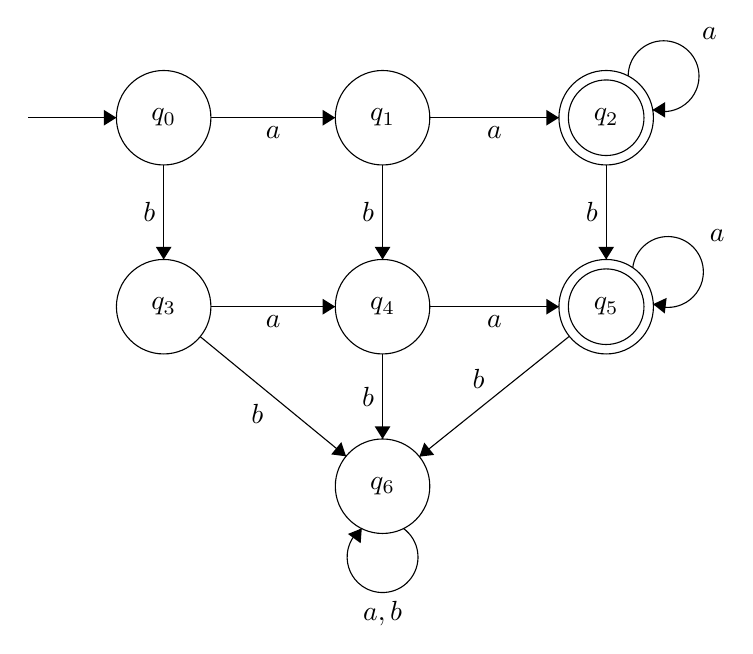
\begin{tikzpicture}[scale=0.2]
		\tikzstyle{every node}+=[inner sep=0pt]
		\draw [black] (13.1,-16.5) circle (3);
		\draw (13.1,-16.5) node {$q_0$};
		\draw [black] (27,-16.5) circle (3);
		\draw (27,-16.5) node {$q_1$};
		\draw [black] (41.2,-16.5) circle (3);
		\draw (41.2,-16.5) node {$q_2$};
		\draw [black] (41.2,-16.5) circle (2.4);
		\draw [black] (13.1,-28.5) circle (3);
		\draw (13.1,-28.5) node {$q_3$};
		\draw [black] (27,-28.5) circle (3);
		\draw (27,-28.5) node {$q_4$};
		\draw [black] (41.2,-28.5) circle (3);
		\draw (41.2,-28.5) node {$q_5$};
		\draw [black] (41.2,-28.5) circle (2.4);
		\draw [black] (27,-39.9) circle (3);
		\draw (27,-39.9) node {$q_6$};
		\draw [black] (16.1,-16.5) -- (24,-16.5);
		\fill [black] (24,-16.5) -- (23.2,-16) -- (23.2,-17);
		\draw (20.05,-17) node [below] {$a$};
		\draw [black] (30,-16.5) -- (38.2,-16.5);
		\fill [black] (38.2,-16.5) -- (37.4,-16) -- (37.4,-17);
		\draw (34.1,-17) node [below] {$a$};
		\draw [black] (42.596,-13.858) arc (179.87911:-108.12089:2.25);
		\draw (47.26,-11.16) node [right] {$a$};
		\fill [black] (44.15,-16) -- (44.95,-16.5) -- (44.95,-15.5);
		\draw [black] (4.5,-16.5) -- (10.1,-16.5);
		\fill [black] (10.1,-16.5) -- (9.3,-16) -- (9.3,-17);
		\draw [black] (13.1,-19.5) -- (13.1,-25.5);
		\fill [black] (13.1,-25.5) -- (13.6,-24.7) -- (12.6,-24.7);
		\draw (12.6,-22.5) node [left] {$b$};
		\draw [black] (16.1,-28.5) -- (24,-28.5);
		\fill [black] (24,-28.5) -- (23.2,-28) -- (23.2,-29);
		\draw (20.05,-29) node [below] {$a$};
		\draw [black] (30,-28.5) -- (38.2,-28.5);
		\fill [black] (38.2,-28.5) -- (37.4,-28) -- (37.4,-29);
		\draw (34.1,-29) node [below] {$a$};
		\draw [black] (27,-19.5) -- (27,-25.5);
		\fill [black] (27,-25.5) -- (27.5,-24.7) -- (26.5,-24.7);
		\draw (26.5,-22.5) node [left] {$b$};
		\draw [black] (41.2,-19.5) -- (41.2,-25.5);
		\fill [black] (41.2,-25.5) -- (41.7,-24.7) -- (40.7,-24.7);
		\draw (40.7,-22.5) node [left] {$b$};
		\draw [black] (42.887,-26.034) arc (173.35104:-114.64896:2.25);
		\draw (47.75,-23.98) node [right] {$a$};
		\fill [black] (44.18,-28.34) -- (44.92,-28.93) -- (45.04,-27.94);
		\draw [black] (15.42,-30.4) -- (24.68,-38);
		\fill [black] (24.68,-38) -- (24.38,-37.1) -- (23.74,-37.88);
		\draw (19.04,-34.69) node [below] {$b$};
		\draw [black] (27,-31.5) -- (27,-36.9);
		\fill [black] (27,-36.9) -- (27.5,-36.1) -- (26.5,-36.1);
		\draw (26.5,-34.2) node [left] {$b$};
		\draw [black] (38.86,-30.38) -- (29.34,-38.02);
		\fill [black] (29.34,-38.02) -- (30.28,-37.91) -- (29.65,-37.13);
		\draw (33.09,-33.71) node [above] {$b$};
		\draw [black] (28.323,-42.58) arc (54:-234:2.25);
		\draw (27,-47.15) node [below] {$a,b$};
		\fill [black] (25.68,-42.58) -- (24.8,-42.93) -- (25.61,-43.52);
		\end{tikzpicture}
	\end{center}
	The above DFA shows that for any string that contains more than 1 `$b$', then machine goes to a regular state and stays there. If the string contains 1 or less `$b$', and 2 or more `$a$', the machine goes to an accept state. 

	\newpage
	\subsubsection*{Problem 3}
	Given the languages $A$ and $B$, and $ C = \{ w \in A \mid w \in B \} $, we need to prove or disprove that if $ A $ and $ B $ are regular languages, then $ C $ is also a regular language.

	By definition, $C$ is the language that consists of all the strings $w$ that belong to both $A$ and $B$. So $C = A \cap B$. 

	If $A$ and $B$ are regular languages, then there must exist some finite automata that recognizes them. Let $M_1$ and $M_2$ be the DFAs that recognize $A$ and $B$ respectively. Then: \\ 
	\hspace*{5mm} - $M_1 = (Q, \Sigma, \delta_A, q_o, F_A)$ recognizes A \\
	\hspace*{5mm} - $M_2 = (R, \Sigma, \delta_B, r_o, F_B)$ recognizes B 
	
	Then we can construct a DFA $M_3$ for $C$ that keeps track of the pair of states $(q_i, r_j)$, where $q_i \in Q$ and $r_j \in R$. In this construction, the states of the new DFA are pairs of states from the $A$ and $B$, that is, the Cartesian Product of the two languages \vspace*{-2mm} $$ Q \times R = \{ (q, r) \mid q \in Q \text{ and } r \in R \} $$

	Then $M_3 = (Q \times R, \sum, \delta, (q_o, r_o), F_A \times F_B)$. \\ For $M_3$, \vspace*{-3mm} 
	\begin{itemize}
		\item[-] Set of states $Q \times R $, the Cartesian Product of $Q$ and $R$ to include all pairs of states in both the machines as mentioned above. \vspace*{-2mm}
		\item[-] $\sum$ remains the same as the input alphabet. \vspace*{-2mm}
		\item[-] We have the transition function $\delta$ defined as \vspace*{-2mm}$$ \delta((q, r), a) = (\delta_A(q, a), \delta_B(r, a)) \;\; \forall q, r \in Q, R \text{ and } \forall a \in \sum $$ \vspace*{-8mm}
		\item[-] The start state is $ (q_o, r_o) $ which is the pair of start states of $M_1$ and $M_2$. \vspace*{-2mm}
		\item[-] The set of accept states is again the Cartesian Product of the accept states of $M_1$ and $M_2$, that is, all pairs of states $(q_f, r_f)$ where $q_f \in F_A$ and $r_f \in F_B$.
	\end{itemize}
	Therefore, by this construction of $M_3$, we have created a DFA that would only reach an accepting state if both, $M_1$ and $M_2$ reach the accept state. Therefore, the string would have to be accepted by both $M_1$ and $M_2$. Hence, for any arbitrary string $w$ that is accepted by $M_3$, $w \in A$ and $w \in B$. 

	Hence, if $A$ and $B$ are regular languages, then we can construct a DFA to recognize $ C = \{ w \in A \mid w \in B \} $, therefore, $C$ is also a regular language. 

	If there are no strings common to both $A$ and $B$, then $C$ will be an empty language, meaning it will only consist of the empty string $ \varepsilon $. Then $ C = \{ \varepsilon \} $ which is also a regular language as again a DFA can be constructed with only 1 state as both the start and accept state. 
	
	Therefore $C$ is a regular language.
	\begin{flushright}
		$\blacksquare$
	\end{flushright}

	\newpage
	\subsubsection*{Problem 4}
	Given the regular languages $A$ and $B$, $ A\smile_a B = \{ u\in A \mid \exists v\in B \ni n_a(u) = n_a(v) \} $. This operation takes two languages $A$, and $B$, and produces a new language that contains all strings $u \in A$ that have the same number of occurrences of $a$ as some string $v \in B$.
	
	Let $ C $ be the language obtained by the operation $ A\smile_a B $. Then $ C = A \smile_a B$.

	If $A$ and $B$ are two regular langauges, then there must exist some finite automata that recognizes them. Let $M_1$ and $M_2$ be the DFAs that recognize $A$ and $B$ respectively. Then: \\
	\hspace*{5mm} - $M_1 = (Q, \Sigma, \delta_A, q_o, F_A)$ recognizes A \\
	\hspace*{5mm} - $M_2 = (R, \Sigma, \delta_B, r_o, F_B)$ recognizes B 
	
	Then we can construct an NFA $M_C$ that recognizes $C$ as follows. To decide whether $ u \in A $ for some arbitrary string $u$, and in parallel nondeterministically guess some string $v \in B$ such that $v$ contains the same number of $ a $'s in $u$. Then $ M_C = \{ Q, \sum, \delta, q_o, F \} $ where: \vspace*{-2mm}
	\begin{enumerate}
		\item $ Q = Q_1 \times Q_2 $, the Cartesian Product of the states of $M_1$ and $M_2$. \vspace*{-2mm}
		\item $ \sum $ remains the same as the input alphabet. \vspace*{-2mm}
		\item $ q_o = q_o $ \vspace*{-2mm}
		\item $ F = F_A \times F_B $ \vspace*{-2mm}
		\item $\delta((q, r), s)$ where $ q \in Q, r \in R, s \in \sum_\varepsilon $,\[ 
            \delta((q, r) s) = \left\{ 
                \begin{array}{l l}
                    \{ \delta_A(q, s), \delta_B(r, s) \},& s = a \\ 
					\{ \delta_A(q, s), r \},& s = b \\
					\{ q, \delta_B(r, s) \},& s = \varepsilon \\
                \end{array}
             \right.     
        \]
	\end{enumerate} 
	The machine must have a parir of all states that exist in $A$ and $B$, that is, the Cartesian Product of the two languages, the start state same as $ q_o $, accept states $ F_A \times F_B$. \\ The transition function is defined such that it has a pair of states, and an alphabet; \vspace*{-2mm}\begin{enumerate}
		\item if the current alphabet is $a$, then it moves on to the next state in $A$, and the next state in $B$, which means that the NFA is now trying to guess a string $v \in B$ that has the same number of occurrences of $a$ as the current input string and the previous input alphabet \vspace*{-2mm}
		\item if the current alphabet is $b$, then the NFA moves on to the next state in $A$ while remaining in the same state in $B$ which again means that the NFA is trying to guess a string $v \in B$ that has the same number of occurrences of $a$ as the current input string and the previous input alphabet, however, it does not change its state in $B$ since we are concerned with the number of occurrences of $a$ \vspace*{-2mm}
		\item if we have an $ \varepsilon $ or an empty string, then it moves on to the next state in $B$ while remaining in the same state in $A$
	\end{enumerate}

	Then the NFA $M_C$ accepts a string if and only if $\forall u \in A $, $ \exists v \in B $ such that $ n_a(u) = n_a(v) $. Again this claim can be proved by showing that the language of $M_C$ is a subset of the language of $ A \smile_a B $ and vice versa.
	
	Suppose $M_C$ accepts a string $s$, meaning that it reaches the accept state when processing $s$. We defined the accept states $F$ as a pair of accept states from $ M_A $ and $ M_B $, i.e., $ (q_f, r_f) $ where $ q_f \in F_A, r_f \in F_B $. For each alphabet $s_i$ in $s$, the transition function ensures that the NFA moves to the next state in $A$ and $B$ if $s_i = a$, and moves to the next state in $A$ while remaining in the same state in $B$ if $s_i = b$. This means that the NFA is guessing a string $v \in B$ that has the same number of occurrences of $a$ as the current input string and the previous input alphabet. If the NFA reaches the accept state, it implies that $M_A$ also reaches the accept state $ q_f \in F_A $ after processing a substring $u$ of $s$, and $M_B$ reaches an accept state $ r_f \in F_B $ after processing a substring $v$ of $s$. Crucially, since $M_C$ accepts $s$, there must be a sequence of transitions in $M_C$ that correspond to reading the alphabets in $s$ such that $ n_a(u) = n_a(v) $ since for each alphabet `$a$' in $s$, $M_C$ consumes one `$a$' in both machines, and for each alphabet `$b$' in $s$, $M_C$ consumes one `$b$' in $M_B$. Hence $ n_a(u) = n_a(v) $, therefore, $L(M_C) \subseteq A \smile_a B$. 
	% If the NFA reaches the accept state, then it means that the string $v$ that it guessed has the same number of occurrences of $a$ as the current input string and the previous input alphabet.
	
	Now consider strings $u \in A$ and $v \in B$, such that $ n_a(u) = n_a(v) $. Then we can construct a string $s$ from $u$ and $v$ such that $ s \in A \smile_a B $ by the definition of the smile operation. Then $s$ is some concatenation of $u$ and $v$. When $M_C$ processes $s$, for each alphabet `$a$' in $s$, $M_C$ consumes one `$a$' in both machines, and for each alphabet `$b$' in $s$, $M_C$ consumes one `$b$' in $M_B$. Hence $M_C$ reaches the accept state in the final state of $M_A$ and $M_B$ both which corresponds to $ q_f \in F_A $ and $ r_f \in F_B $ respectivel. Therefore, $A \smile_a B \subseteq L(M_C)$. 

	Hence, the class of regular languages is closed under $\smile_a$.
	\begin{flushright}
		$\blacksquare$
	\end{flushright}

\end{solution}
\end{questions}

\end{document}

%%% Local Variables:
%%% mode: latex
%%% TeX-master: t
%%% End:
